\newpage
\changeindent{0cm}
\section{ショートカット探索}
\label{sec:pred}
\changeindent{2cm}

\begin{figure}[t]
  \begin{center}
    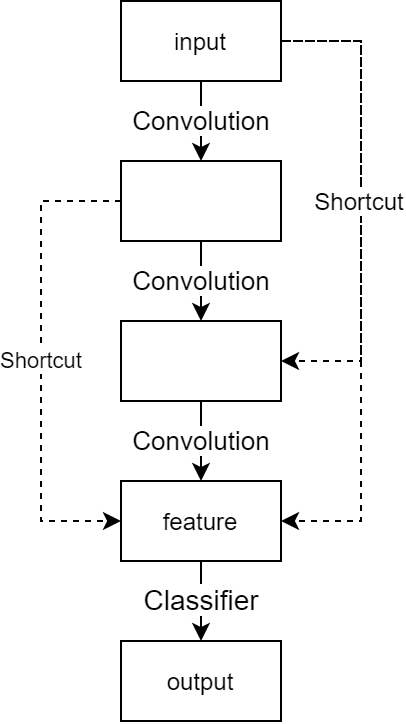
\includegraphics[clip,width=6cm]{./fig/03.pred/image.png}
  \end{center}
  \caption{ショートカット概念図}
  \label{fig:image}
\end{figure}

DARTSで柔軟なアーキテクチャを探索することを実験の目的とし, 構造探索タスクとして
深層畳み込みネットワークのVGG19\cite{Simonyan15}の
ショートカット接続\cite{mao2016image}を考える.
図 \ref{fig:image} のように, ショートカット接続は,
畳み込み部において 1つ以上特徴を飛ばした接続とする.
VGG19は分岐がない単純なネットワーク構造であるため, ベースモデルに適しているとして選択した.

VGG19は16層の畳み込み層と3層の線形結合層を持つ.
表 \ref{tab:vgg} は, VGG19の畳み込みニューラルネットワーク
(Convolutional Neural Network: CNN) 部分の構造を示している.
構成する関数は, フィルターサイズが 3 x 3 の畳み込み層(Conv2d),
Batch Normalization(BN)\cite{Ioffe2015BatchNA},
活性化関数(Rectified Linear Unit: ReLU),
ストライドが 2 の Max Pooling (MaxPool)である.
このVGG19に対し層を飛ばして接続するショートカットの数と位置を求め,
性能を向上させることを目的とする.

\begin{table}[t]
  \begin{center}
    \caption{VGG19 の構造}
		\vspace{-1mm}
    例として入力する画像を(32, 32, 3)次元としている.
		\vspace{1mm}
		\vspace{3mm}
    \begin{tabular}{|c|c|c|l|}
    \hline
    \textbf{index} & \textbf{image size} & \textbf{channels} & \multicolumn{1}{c|}{\textbf{applied function}} \\ \hline
    input & 32 x 32 & 3   & \multicolumn{1}{c|}{-}         \\ \hline
    1     & 32 x 32 & 64  & 3x3\_Conv2d, BN, ReLU          \\ \hline
    2     & 16 x 16 & 64  & 3x3\_Conv2d, BN, ReLU, MaxPool \\ \hline
    3     & 16 x 16 & 128 & 3x3\_Conv2d, BN, ReLU          \\ \hline
    4     & 8 x 8   & 128 & 3x3\_Conv2d, BN, ReLU, MaxPool \\ \hline
    5     & 8 x 8   & 256 & 3x3\_Conv2d, BN, ReLU          \\ \hline
    6     & 8 x 8   & 256 & 3x3\_Conv2d, BN, ReLU          \\ \hline
    7     & 8 x 8   & 256 & 3x3\_Conv2d, BN, ReLU          \\ \hline
    8     & 4 x 4   & 256 & 3x3\_Conv2d, BN, ReLU, MaxPool \\ \hline
    9     & 4 x 4   & 512 & 3x3\_Conv2d, BN, ReLU          \\ \hline
    10    & 4 x 4   & 512 & 3x3\_Conv2d, BN, ReLU          \\ \hline
    11    & 4 x 4   & 512 & 3x3\_Conv2d, BN, ReLU          \\ \hline
    12    & 2 x 2   & 512 & 3x3\_Conv2d, BN, ReLU, MaxPool \\ \hline
    13    & 2 x 2   & 512 & 3x3\_Conv2d, BN, ReLU          \\ \hline
    14    & 2 x 2   & 512 & 3x3\_Conv2d, BN, ReLU          \\ \hline
    15    & 2 x 2   & 512 & 3x3\_Conv2d, BN, ReLU          \\ \hline
    16    & 1 x 1   & 512 & 3x3\_Conv2d, BN, ReLU, MaxPool \\ \hline
    \end{tabular}
    \label{tab:vgg}
  \end{center}
\end{table}


モデル中の潜在的特徴は高さ・幅・チャンネル数を持つデータであるが,
特徴の次元は場所によって異なるため, ショートカットは次元を変換する必要がある.
したがってショートカット関数は以下のように設定した.
\begin{enumerate}
  \item 次元が同じ場合:恒等関数
  \item チャンネル数が違う場合:Pointwise Convolution
  \item 高さと幅が半分の場合:Factorized Reduce
  \item それ以外の場合:ショートカットを定義しない
\end{enumerate}
Pointwise Convolutionは, 要素ごとの畳み込みでチャンネル数を調整する.
Factorized Reduceは, 畳み込み層を偶数列と奇数列の 2枚 用いることで, 情報の損失を防ぎつつ特徴次元を半分にすることができる.

ショートカットに使用する関数の制限によってショートカット位置の候補は61であるため,
探索空間は$2^{61}$である.
演算子の種類は固定することで, アーキテクチャ $\alpha$ は畳み込み部に相当するグラフの重みをもつ隣接行列と定義した.


%4.1
\changeindent{0cm}
\subsection{提案手法:DARTS}
\label{sec:pred.01}
\changeindent{2cm}

DARTSでネットワーク構造を探索するときの, 学習の手順は
\begin{enumerate}
  \item 探索:アーキテクチャ $\alpha$ の訓練
  \item 構成:$\alpha$ からネットワークを構成
  \item 評価:得られたネットワークをバックプロパゲーションにより訓練し, テストデータで性能を評価
\end{enumerate}
の 3段階から成る.

\subsubsection{探索}

探索段階では, 勾配降下法によって $\alpha$ の更新を行う.
このとき探索用のネットワークは, ショートカットの本数も探索するため,
$\alpha$ に対する重み補正 $\beta$ を用いて (\ref{equ:cut}) 式 で定義する.
\begin{equation}
  \label{equ:cut}
  x_i = f^{\mathrm{c}}_{i-1, i}(x_{i-1}) + \beta_i \sum_{j \in S_i} \alpha_{ij} f^{\mathrm{s}}_{j, i} (x_j)
\end{equation}
ここで $f^{\mathrm{c}}(・)$, $f^{\mathrm{s}}(・)$ は, VGGの畳み込み関数とショートカット関数,
$S_i$ はノード $i$ とショートカットで接続する先行(predecessor)ノードのインデックス集合である.

ただし$\beta=0$で勾配の更新ができなくなるので,
\begin{equation}
  \label{equ:beta}
  \hat{\beta} = \begin{cases}
    \exp(\beta - 1) & (\beta \leq 1) \\
    \log(\beta) + 1 & (\mathrm{otherwise})
  \end{cases}
\end{equation}
で0とならないように補正した $\hat{\beta}$ を用いた.

\subsubsection{構成}

構成段階では, 探索段階で得られた $\alpha$ から具体的なネットワークをサンプリングする.
$\alpha$ の値に対する, ネットワークの構成手法はいくつか考えられるため,
\begin{itemize}
  \item 構成手法A : predecessorsの中で大きい順に採択
  \item 構成手法B : 閾値以上のエッジを採択
\end{itemize}
の 2通りの手法を設定した.
% (predecessorsはあるノードに接続している前のノードの集合)

\subsubsection{評価}
評価段階では, 構成段階で得られたネットワークを学習し,
最大の正答率をネットワークの性能とする.
このときのパラメータは, グリッドサーチによる最適化API の optuna \cite{akiba2019optuna}
で事前学習した結果から設定する.


\changeindent{0cm}
\subsubsection{実験概要}
\label{sec:pred.01_03}
\changeindent{2cm}

提案手法:DARTSの実験を 実験1 とする.
表 \ref{tab:setting_exp}, \ref{tab:exp2/eval} に実験1の探索段階と評価段階の実験設定を示す.
探索段階は先行研究のDARTSの設定を参考に, 評価段階はoptunaで最適化した値を使用した.
$\alpha$ の Optimizer はAdam\cite{Kingma2015AdamAM}で,
評価段階では, 訓練中に学習率を変化させる Scheduler\cite{Loshchilov2017SGDRSG}を用いた.

データセットは, 32 pixel * 32 pixel * 3 channel の訓練画像を 50000枚 持つ CIFAR-10\cite{cifar10} を利用して,
10クラス分類問題を解いた.

探索 epoch 数は, 150 epochとし, 50 epochごとにその時点の $\alpha$ の性能を評価した.
構成段階では手法A, Bに加えて比較のため,
ショートカット数が同じとなる条件でランダムに選択する手法でも実験する.
各手法において10回試行して統計的な性能を比較した.

\begin{table}[tb]
  \begin{center}
    \caption{実験1 : 探索段階の設定}
  	\vspace{3mm}
    \begin{tabular}{|c|c|} \hline
      Step & Architecture Search \\ \hline\hline
      Loss & Cross Entropy Loss \\ \hline
      batch size & 64 \\ \hline
      Optimizer($w$) & SGD(lr=0.001, momentum=0.9) \\ \hline
      Optimizer($\alpha$) & Adam(lr=0.003, $\beta$=(0.5, 0.999)) \\ \hline
      epoch & 150\\ \hline
      train data & 25000\\ \hline
      valid data & 25000\\ \hline
      test data &  10000\\ \hline
    \end{tabular}
    \label{tab:setting_exp}
  \end{center}
\end{table}

\begin{table}[tb]
  \begin{center}
    \caption{実験1 : 評価段階の設定}
  	\vspace{3mm}
    \begin{tabular}{|c|c|} \hline
      Step & Evaluation \\ \hline\hline
      Loss & Cross Entropy Loss \\ \hline
      batch size & 64 \\ \hline
      Optimizer($w$) & SGD(lr=0.0090131, momentum=0.9) \\ \hline
      Scheduler($w$) & Step($\gamma$=0.23440, stepsize=100) \\ \hline
      epoch & 150\\ \hline
      train data & 50000\\ \hline
      test data &  10000\\ \hline
    \end{tabular}
    \label{tab:exp2/eval}
  \end{center}
\end{table}


\clearpage\newpage
\changeindent{0cm}
\subsection{提案手法:DARTS+TDGA}
\label{sec:pred.02}
\changeindent{2cm}

\begin{figure}[t]
  \begin{center}
    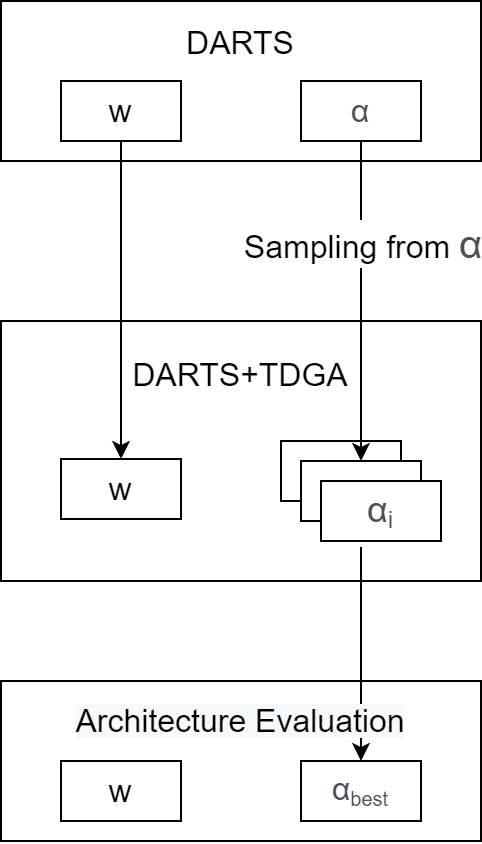
\includegraphics[clip,width=6cm]{./fig/03.pred/datdga.png}
  \end{center}
  \caption{提案手法:DARTS+TDGA 概念図}
  \label{fig:image_ga}
\end{figure}

実験1では $\alpha$ の学習程度によって重み $w$ の学習しやすさに偏りがあったため,
収束するグラフ構造にばらつきが見られた.

そこで実験1から得られた構造探索のための実験設定をもとに,
個体表現を $\alpha$ とした遺伝的アルゴリズムによって,
アーキテクチャを複数同時に管理, 最適化し,
個体群の多様性を維持しつつ, 安定的なネットワーク構造の学習を図った.
単純に個体数を増やすと計算コストが定数倍されるため,
重み $w$ は全体で共有する One-Shot モデルを利用することで高速化した.


\subsubsection{多様性項の拡張}
(\ref{eq:Entropy}) 式では, 多様性の計算にエントロピーを利用していたが,
個体 $\alpha$ は実数値の行列であるためエントロピーは計算できない.

\begin{equation}
H = \sum_{k \in \mathcal{P}} \sqrt{\mathrm{MSE}(\alpha_k, \bar{\alpha})} \label{eq:Entropy-new}
\end{equation}

そこで行列の各要素の標準偏差の平均として, $H$ の実数値拡張をした.


\subsubsection{実験手順}
実験は3段階からなり, 事前学習したDARTSから, $w$, $\alpha$を引き継ぎ,
TDGAで再探索し, 得られた最良個体のアーキテクチャを学習して性能を評価する.
図 \ref{fig:image_ga} に$w$, $\alpha$の関係を示す.

\begin{enumerate}
  \item 事前学習
  \item アーキテクチャ再探索
  \item 性能評価
\end{enumerate}

\subsubsection{事前学習}
DARTSをする.
softmaxからsigmoidへ.
(ここに説明を入力)


\subsubsection{アーキテクチャ再探索}

以下に TDGA をベースとして, DARTSの学習ステップの追加と多様性項の実数値拡張をした提案手法のアルゴリズム

\begin{itemize}
  \item 提案手法1. DARTS + TDGA($w$, $\alpha$)
  \item 提案手法2. DARTS + TDGA($\alpha$)
  \item 提案手法3. DARTS + TDGA
\end{itemize}

\noindent
を アルゴリズム \ref{alg1}, \ref{alg2}, \ref{alg3} に示す.
アルゴリズム \ref{alg1} をベースとして, DARTSによる勾配更新のステップを無効にすることで,
DARTSがTDGAの学習に与える影響をみる.

\begin{algorithm}
  \caption{提案手法1. DARTS + TDGA($w$, $\alpha$)}
  \label{alg1}
  \begin{enumerate}
    \item DARTSで事前学習したモデルの重みを引き継いだ初期個体を生成
    \item エリート個体選択
    \item 重み $w$ を $\displaystyle \nabla_\alpha \mathcal{L}_{\mathrm{train}}(w, \bar{\alpha})$ で更新
    \item 個体 $\alpha_i$ を $\displaystyle \nabla_\alpha \mathcal{L}_{\mathrm{valid}}(w, \alpha_i)$ で更新
    \item 適応度 $\displaystyle \mathcal{L}_{\mathrm{test}}(w, \alpha_i)$ で個体 $\alpha_i$ を評価
    \item 交叉で子個体群生成
    \item 親個体群と子個体群の突然変異
    \item エリート個体と親個体群, 子個体群に熱力学的選択によって次世代とする
    \item 収束するまで 2. に戻る
  \end{enumerate}
\end{algorithm}


\begin{algorithm}
  \caption{提案手法2. DARTS + TDGA($\alpha$)}
  \label{alg2}
  \begin{enumerate}
    \item DARTSで事前学習したモデルの重みを引き継いだ初期個体を生成
    \item エリート個体選択
    \item 個体 $\alpha_i$ を $\displaystyle \nabla_\alpha \mathcal{L}_{\mathrm{valid}}(w, \alpha_i)$ で更新
    \item 適応度 $\displaystyle \mathcal{L}_{\mathrm{test}}(w, \alpha_i)$ で個体 $\alpha_i$ を評価
    \item 交叉で子個体群生成
    \item 親個体群と子個体群の突然変異
    \item エリート個体と親個体群, 子個体群に熱力学的選択によって次世代とする
    \item 収束するまで 2. に戻る
  \end{enumerate}
\end{algorithm}

\begin{algorithm}
  \caption{提案手法3. DARTS + TDGA}
  \label{alg3}
  \begin{enumerate}
    \item DARTSで事前学習したモデルの重みを引き継いだ初期個体を生成
    \item エリート個体選択
    \item 適応度 $\displaystyle \mathcal{L}_{\mathrm{test}}(w, \alpha_i)$ で個体 $\alpha_i$ を評価
    \item 交叉で子個体群生成
    \item 親個体群と子個体群の突然変異
    \item エリート個体と親個体群, 子個体群に熱力学的選択によって次世代とする
    \item 収束するまで 2. に戻る
  \end{enumerate}
\end{algorithm}


% $P$は個体群,
% $\bar{\alpha}$ は各個体の平均,
% $\alpha_$ は実験1で有効だった構成手法Bで隣接行列にサンプリングした $\alpha$ である.


\subsubsection{性能評価}

性能評価の段階では, 提案手法による探索結果をもとに,
学習後最終世代の個体の性能を実験1と同じ条件で学習し評価した.


\changeindent{0cm}
\subsubsection{実験概要}
\label{sec:pred.02_03}
\changeindent{2cm}

提案手法:DARTS+TDGAの実験を 実験2 とする.

表 \ref{tab:setting_pretrain} には事前学習の設定を示した.
実験1 の設定を継承しつつ,
モデルの重み $w$ はImage Netで訓練された事前学習の重みを畳み込み層の部分に適用した.

表 \ref{tab:setting_darts}, \ref{tab:setting_ga}にモデルとGAの実験設定を示した.
初期収束を防ぐため, 交叉にはエッジに相当する遺伝子座ごとに 0.8 の確率で操作する一様交叉を使用した.
突然変異には遺伝子座ごとに 0.1 の確率で $\mu=0$, $\gamma=0.2$ となるガウス分布からの摂動を与えた.
交叉と突然変異の操作確率は, 個体ごとの確率で, それぞれは独立であり, 交叉の後に突然変異をした.

% ここで 0.5 Page

\begin{table}[tb]
  \begin{center}
    \caption{実験2 : 事前学習の設定}
  	\vspace{3mm}
    \begin{tabular}{|c|c|} \hline
      Optimizer($w$) & SGD(lr=0.001, momentum=0.9) \\ \hline
      Optimizer($\alpha$) & Adam(lr=0.0005, $\beta$=(0.5, 0.999)) \\ \hline
      Loss & Cross Entropy Loss \\ \hline
      batch size & 64 \\ \hline
      train data & 25000\\ \hline
      valid data & 25000\\ \hline
      test data &  10000\\ \hline
      epoch & 150\\ \hline
    \end{tabular}
    \label{tab:setting_pretrain}
  \end{center}
\end{table}

\begin{table}[t]
  \begin{center}
    \caption{実験2 : DARTS+TDGAの設定 (DARTS)}
  	\vspace{3mm}
    \begin{tabular}{|c|c|} \hline
      Optimizer($w$) & SGD(lr=0.001, momentum=0.9) \\ \hline
      Optimizer($\alpha$) & Adam(lr=0.001, $\beta$=(0.5, 0.999)) \\ \hline
      Loss & Cross Entropy Loss \\ \hline
      batch size & 64 \\ \hline
      train data & 25000\\ \hline
      valid data & 25000\\ \hline
      test data &  2000\\ \hline
    \end{tabular}
    \label{tab:setting_darts}
  \end{center}
\end{table}

\begin{table}[t]
  \begin{center}
    \caption{実験2 : DARTS+TDGAの設定 (TDGA)}
  	\vspace{3mm}
    \begin{tabular}{|c|c|} \hline
      Population & 10 \\ \hline
      Generation & 150 \\ \hline \hline
      Selection & Elite \\ \hline
      Elite \# & 1 \\ \hline
      Selection & TD Select \\ \hline
      Temperature & 1 $\rightarrow$ 0.001 \\ \hline \hline
      Crossover & Uniform Crossover (0.5 / locus) \\ \hline
      Crossover Rate & 0.8 \\ \hline \hline
      Mutation & Gaussian Mutation ($\mu$=0, $\sigma$=0.2, 0.2 / locus)\\ \hline
      Mutation Rate & 0.2 \\ \hline
    \end{tabular}
    \label{tab:setting_ga}
  \end{center}
\end{table}

\begin{table}[t]
  \begin{center}
    \caption{実験2 : ネットワーク評価の設定}
  	\vspace{3mm}
    \begin{tabular}{|c|c|} \hline
      Optimizer($w$) & SGD(lr=0.009, momentum=0.9) \\ \hline
      Scheduler($w$) & Step($\gamma$=0.2344, step epoch=100) \\ \hline
      Loss & Cross Entropy Loss \\ \hline
      batch size & 64 \\ \hline
      train data & 50000\\ \hline
      test data &  10000\\ \hline
      epoch & 150\\ \hline
    \end{tabular}
    \label{tab:setting_eval}
  \end{center}
\end{table}
